

\pgfdeclarelayer{bg}
\pgfsetlayers{bg,main}

\begin{figure}
    \centering
    \begin{tikzpicture}
        \tikzstyle{every node}=[node distance=4cm,minimum height=0.8cm]
        % loss functions
        \node[draw,fill=black,minimum height=0.2cm,circle] (lossroot) at (0,0) {};
        \node[above of=lossroot, node distance=1cm] {Loss Functions};

        % regression
        \node[draw,fill=black,minimum height=0.2cm,circle, below left of=lossroot] (regressionroot)  {};
        \draw[->] (lossroot) -- node[fill=white] {Regression} (regressionroot);

        \node[draw,below left of=regressionroot] (mse)  {Squared Error};
        \draw[->] (regressionroot) -- node[fill=white] {Reals} (mse.north);
        \node[draw,below right of=regressionroot] (amse) {Squared Angular Error};
        \draw[->] (regressionroot) -- node[fill=white] {Angles} (amse.north);

        % parameter estimation
        \node[draw,fill=black,minimum height=0.2cm,circle,right of=amse] (param) {};
        \draw[->] (lossroot) -- node[fill=white] {Parameter Estimation} (param);
        \node[draw,below of=param] (gaussian) {Gaussian NLL};
        \draw[->] (param) -- node[fill=white] {Reals} (gaussian.north);

        \node[draw,below right of=param] (angles) {Von-Mises NLL};
        \draw[->] (param) -- node[fill=white] {Angles} (angles.north);

        \node[draw,below left of=param] (softmax) {Categorical NLL};
        \draw[->] (param) -- node[fill=white] {Categorical} (softmax.north);

    \end{tikzpicture}
    \vspace{1cm}
    \captionsetup{parskip=7pt}
    \caption[Ontology of loss functions.]{We can split loss functions into two categories.

    In the former, the loss function has the form of an error function. When minimizing this function, the model learns to output the expected value of the posterior $\E\left[p(y \mid x)\right]$ of the output $y$ given the input $x$. This is called a regression or maximum-a-posteriori (MAP) task.

    In the latter, the loss function has the form of a negative-log-likelihood (NLL) function. The model outputs the parameters of a probability distribution, and the loss function is the negative log-likelihood of the data under that distribution. This includes the case of categorical NLL (also called categorical cross-entropy), where the model outputs a probability distribution over a discrete set of classes.

    Models trained with a NLL loss learn to output an explicit posterior distribution $p(y \mid x)$, given a fixed functional form for $p$, such as a Gaussian, mixture of Gaussians, Categorical, Von-Mises, etc. Depending on the task, and output format, different functional forms for $p$ may be appropriate.}
    \label{fig:ontology-loss}
\end{figure}


\begin{figure}
    \centering
    \begin{tikzpicture}
        \tikzstyle{every node}=[node distance=3.5cm,minimum height=0.8cm]
        \node[draw,fill=black,minimum height=0.2cm,circle] (taskroot) at (0,0) {};
        \node[above of=taskroot, node distance=1cm] {Dataset Type};

        % unlabeled data
        \node[draw,fill=black,minimum height=0.2cm,circle, below right of=taskroot] (unlabeled)  {};
        \draw[->] (taskroot) -- node[fill=white] {Un-labeled} (unlabeled);

        % representation learning
        \node[draw, below left of=unlabeled] (representation)  {Representation Learning};
        \draw[->] (unlabeled) -- (representation.north);

        % sequence prediction
        \node[draw, below right of=unlabeled] (nexttoken) {Sequence Prediction};
        \draw[->] (unlabeled) -- (nexttoken.north);

        % labeled
        \node[draw,fill=black,minimum height=0.2cm,circle,left of=representation] (labeled) {};
        \draw[->] (taskroot) -- node[fill=white] {Labeled} (labeled);

        % classification
        \node[draw,below left of=labeled] (classification) {Classification};
        \draw[->] (labeled) -- (classification.north);

        % regression
        \node[draw,below right of=labeled] (regression) {Regression};
        \draw[->] (labeled) -- (regression.north);


    \end{tikzpicture}
    \vspace{1cm}
    \captionsetup{parskip=7pt}
    \caption[Ontology of dataset types]{Basic ontology of dataset types.

    When learning on unlabeled data, the goal is to learn a representation of the data that is useful for some downstream task.

    When learning on data that is explicitly labeled -- the goal is to learn a model that performs well on the task directly.}
    \label{fig:ontology-task}
\end{figure}


\begin{figure}
    \centering
    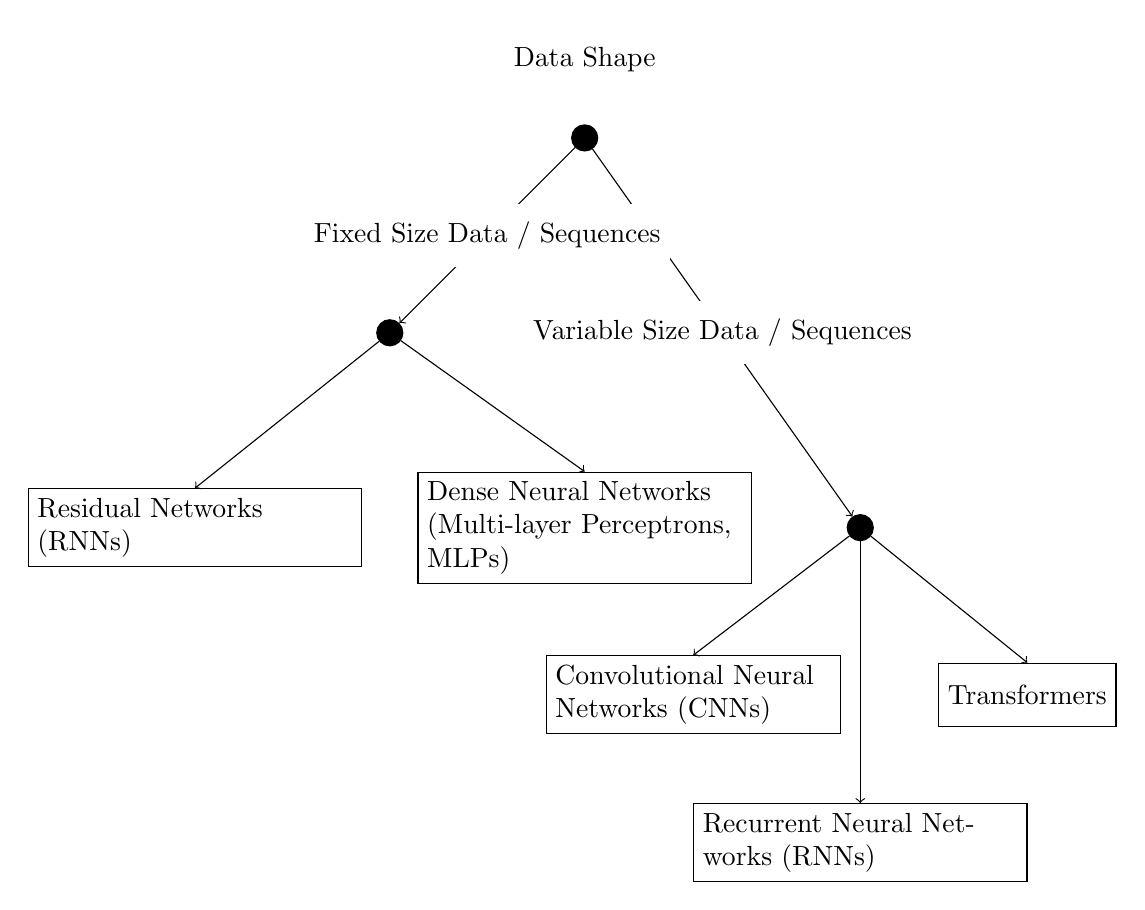
\begin{tikzpicture}
        \tikzstyle{every node}=[node distance=3.5cm,minimum height=0.8cm]
        % data shape
        \node[draw,fill=black,minimum height=0.2cm,circle] (taskroot) at (0,0) {};
        \node[above of=taskroot, node distance=1cm] {Data Shape};

        % fixed input shape
        \node[draw,fill=black,minimum height=0.2cm,circle, below left of=taskroot] (fixed)  {};

        % ResNet
        \node[draw, below left of=fixed,text width=4cm] (resnet)  {Residual Networks (RNNs)};
        \draw[->] (fixed) -- (resnet.north);

        % MLP
        \node[draw, below right of=fixed,text width=4cm] (mlp) {Dense Neural Networks (Multi-layer Perceptrons, MLPs)};
        \draw[->] (fixed) -- (mlp.north);

        % sequence
        \node[draw,fill=black,minimum height=0.2cm,circle,right of=mlp] (sequence) {};
        \draw[->] (taskroot) -- node[fill=white] {Variable Size Data / Sequences} (sequence);

        % this here to draw over above line
        \draw[->] (taskroot) -- node[fill=white] {Fixed Size Data / Sequences} (fixed);

        % CNN
        \node[draw, below left of=sequence,text width=3.5cm, node distance=3cm] (cnn) {Convolutional Neural Networks (CNNs)};
        \draw[->] (sequence) -- (cnn.north);

        % RNN
        \node[draw,below of=sequence,text width=4cm, node distance=4cm] (rnn) {Recurrent Neural Networks (RNNs)};
        \draw[->] (sequence) -- (rnn.north);

        % Transformer
        \node[draw,below right of=sequence, node distance=3cm] (transformer) {Transformers};
        \draw[->] (sequence) -- (transformer.north);

    \end{tikzpicture}
    \vspace{1cm}
    \captionsetup{parskip=7pt}
    \caption[Fixed vs variable input shape]{Neural network variants which support variable input shape.

    Due to their construction, MLPs and ResNets are restricted to a fixed input shape, and so can only be trained and used on data that is of a fixed size, such as tabular data, or data that has been processed into a fixed size by re-sampling, chunking etc.

    RNNs, CNNs and Transformers can accept variable length data, each with their own tradeoffs. They are typically more suitable for data that is naturally of variable size/length, such as text, audio or images.}
    \label{fig:ontology-input-shape}
\end{figure}
